%%%%%%%%%%%%%%%%%%%%%%%%%%%%%%%%%%%%
% Slide options
%%%%%%%%%%%%%%%%%%%%%%%%%%%%%%%%%%%%

% Option 1: Slides with solutions

\documentclass[slidestop,compress,mathserif]{beamer}
\newcommand{\soln}[1]{\textit{#1}}
\newcommand{\solnGr}[1]{#1}

% Option 2: Handouts without solutions

%\documentclass[11pt,containsverbatim,handout]{beamer}
%\usepackage{pgfpages}
%\pgfpagesuselayout{4 on 1}[letterpaper,landscape,border shrink=5mm]
%\newcommand{\soln}[1]{ }
%\newcommand{\solnGr}{ }

%%%%%%%%%%%%%%%%%%%%%%%%%%%%%%%%%%%%
% Style
%%%%%%%%%%%%%%%%%%%%%%%%%%%%%%%%%%%%

\input{../../lec_style.tex}


%%%%%%%%%%%%%%%%%%%%%%%%%%%%%%%%%%%%
% Preamble
%%%%%%%%%%%%%%%%%%%%%%%%%%%%%%%%%%%%

\title[Chp 1: Intro. to data]{Chapter 1: Introduction to data}
\author{OpenIntro Statistics, 4th Edition}
\institute{$\:$ \\ {\footnotesize Slides developed by Mine \c{C}etinkaya-Rundel of OpenIntro. \\
The slides may be copied, edited, and/or shared via the \webLink{http://creativecommons.org/licenses/by-sa/3.0/us/}{CC BY-SA license.} \\
Some images may be included under fair use guidelines (educational purposes).}}
\date{}

%%%%%%%%%%%%%%%%%%%%%%%%%%%%%%%%%%%%
% Begin document
%%%%%%%%%%%%%%%%%%%%%%%%%%%%%%%%%%%%

\begin{document}


%%%%%%%%%%%%%%%%%%%%%%%%%%%%%%%%%%%%
% Title page
%%%%%%%%%%%%%%%%%%%%%%%%%%%%%%%%%%%%

{
\addtocounter{framenumber}{-1} 
{\removepagenumbers 
\usebackgroundtemplate{\includegraphics[width=\paperwidth]{../../OpenIntro_Grid_4_3-01.jpg}}
\begin{frame}

\hfill \includegraphics[width=20mm]{../../oiLogo_highres}

\titlepage

\end{frame}
}
}


%%%%%%%%%%%%%%%%%%%%%%%%%%%%%%%%%%%%
% Sections
%%%%%%%%%%%%%%%%%%%%%%%%%%%%%%%%%%%%

%%%%%%%%%%%%%%%%%%%%%%%%%%%%%%%%%%%%

\section{Case study}

%%%%%%%%%%%%%%%%%%%%%%%%%%%%%%%%%%%%

\begin{frame}
\frametitle{Treating Chronic Fatigue Syndrome}

\begin{itemize}

\item Objective: Evaluate the effectiveness of cognitive-behavior therapy for chronic fatigue syndrome.

\item Participant pool: 142 patients who were recruited from referrals by primary care physicians and consultants to a hospital clinic specializing in chronic fatigue syndrome.

\item Actual participants: Only 60 of the 142 referred patients entered the study. Some were excluded because they didn't meet the diagnostic criteria, some had other health issues, and some refused to be a part of the study.

\end{itemize}

\ct{Deale et. al. \textit{Cognitive behavior therapy for chronic fatigue syndrome: A randomized controlled trial}. The American Journal of Psychiatry 154.3 (1997).}

\end{frame}

%%%%%%%%%%%%%%%%%%%%%%%%%%%%%%%%%%%%

\begin{frame}
\frametitle{Study design}

\begin{itemize}

\item Patients randomly assigned to treatment and control groups, 30 patients in each group:
\begin{itemize}
\item \hl{Treatment}: Cognitive behavior therapy -- collaborative, educative, and with a behavioral emphasis. Patients were shown on how activity could be increased steadily and safely without exacerbating symptoms.
\item \hl{Control:} Relaxation -- No advice was given about how activity could be increased. Instead progressive muscle relaxation, visualization, and rapid relaxation skills were taught.
\end{itemize}

\end{itemize}

\end{frame}

%%%%%%%%%%%%%%%%%%%%%%%%%%%%%%%%%%%%

\begin{frame}
\frametitle{Results}

The table below shows the distribution of patients with good outcomes at 6-month follow-up. Note that 7 patients dropped out of the study: 3 from the treatment and 4 from the control group.

\begin{center}
\begin{tabular}{ll  cc c} 
			&				& \multicolumn{2}{c}{\textit{Good outcome}} \\
\cline{3-4}
			&							& Yes 	& No 	& Total	\\
\cline{2-5}
							&Treatment 	& 19	 	& 8		& 27 	\\
\raisebox{1.5ex}[0pt]{\textit{Group}}	&Control		& 5	 	& 21	 	& 26 \\
\cline{2-5}
							&Total		& 24		& 29		& 53
\end{tabular}
\end{center}

\pause

\begin{itemize}

\item Proportion with good outcomes in treatment group:
\[ 19 / 27 \approx 0.70 \rightarrow 70\% \]

\pause

\item Proportion with good outcomes in control group:
\[ 5 / 26 \approx 0.19 \rightarrow 19\% \]

\end{itemize}

\end{frame}

%%%%%%%%%%%%%%%%%%%%%%%%%%%%%%%%%%%%

\begin{frame}
\frametitle{Understanding the results}

\dq{Do the data show a ``real" difference between the groups?}

\pause

\begin{itemize}

\item Suppose you flip a coin 100 times. While the chance a coin lands heads in any given coin flip is 50\%, we probably won't observe exactly 50 heads. This type of fluctuation is part of almost any type of data generating process.

\item The observed difference between the two groups (70 - 19 = 51\%) may be real, or may be due to natural variation.

\item Since the difference is quite large, it is more believable that the difference is real.

\item We need statistical tools to determine if the difference is so large that we should reject the notion that it was due to chance.

\end{itemize}

\end{frame}

%%%%%%%%%%%%%%%%%%%%%%%%%%%%%%%%%%%%

\begin{frame}
\frametitle{Generalizing the results}

\dq{Are the results of this study generalizable to all patients with chronic fatigue syndrome?}

\pause

These patients had specific characteristics and volunteered to be a part of this study, therefore they may not be representative of all patients with chronic fatigue syndrome. While we cannot immediately generalize the results to all patients, this first study is encouraging. The method works for patients with some narrow set of characteristics, and that gives hope that it will work, at least to some degree, with other patients.


\end{frame}

%%%%%%%%%%%%%%%%%%%%%%%%%%%%%%%%%%%%


%%%%%%%%%%%%%%%%%%%%%%%%%%%%%%%%%%%%

\section{Sampling principles and strategies}

%%%%%%%%%%%%%%%%%%%%%%%%%%%%%%%%%%%%

\subsection{Populations and samples}

%%%%%%%%%%%%%%%%%%%%%%%%%%%%%%%%%%%%

\begin{frame}
\frametitle{Populations and samples}

\twocol{0.5}{0.5}{
\begin{center}
%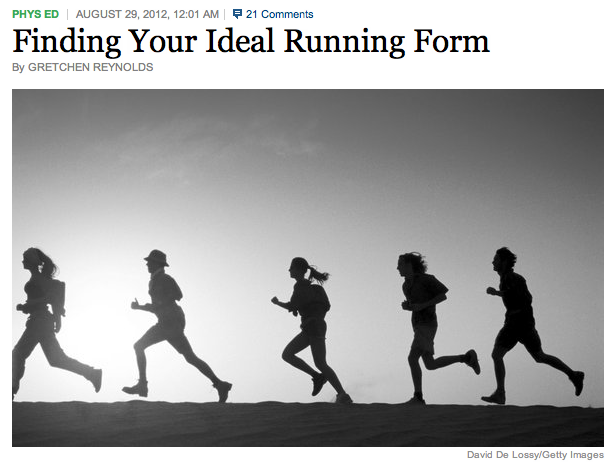
\includegraphics[width=\textwidth]{../../Chp 1/1-3_sampling_principles_strategies/1-3_sampling_principles_strategies/figures/running.png}
\end{center}
\vspace{-0.5cm}
{\tiny \webURL{http://well.blogs.nytimes.com/2012/08/29/finding-your-ideal-running-form}}
}
{
\hl{Research question:} Can people become better, more efficient runners on their own, merely by running? \\

\pause 

\hl{Population of interest:} \soln{\pause All people}
}
\pause 
$\:$ \\
\hl{Sample:} Group of adult women who recently joined a running group

\pause

\hl{Population to which results can be generalized:} \soln{\pause Adult women, if the data are randomly sampled}

\end{frame}

%%%%%%%%%%%%%%%%%%%%%%%%%%%%%%%%%%%%

\subsection{Anecdotal evidence}

%%%%%%%%%%%%%%%%%%%%%%%%%%%%%%%%%%%%

\begin{frame}
\frametitle{Anecdotal evidence and early smoking research}

\begin{itemize}

\item Anti-smoking research started in the 1930s and 1940s when cigarette smoking became increasingly popular. While some smokers seemed to be sensitive to cigarette smoke, others were completely unaffected.

\item Anti-smoking research was faced with resistance based on \hl{anecdotal evidence} such as ``My uncle smokes three packs a day and he's in perfectly good health", evidence based on a limited sample size that might not be representative of the population.

\item It was concluded that ``smoking is a complex human behavior, by its nature difficult to study, confounded by human variability."

\item In time researchers were able to examine larger samples of cases (smokers), and trends showing that smoking has negative health impacts became much clearer.

\end{itemize}

\ct{Brandt, \textit{The Cigarette Century} (2009), Basic Books.}

\end{frame}

%%%%%%%%%%%%%%%%%%%%%%%%%%%%%%%%%%%%

\subsection{Sampling from a population}

%%%%%%%%%%%%%%%%%%%%%%%%%%%%%%%%%%%%

\begin{frame}
\frametitle{Census}

\begin{itemize}

\item Wouldn't it bes better to just include everyone and ``sample" the entire population? 

\begin{itemize}
\item This is called a \hl{census}.
\end{itemize}

\pause

\item There are problems with taking a census:

\begin{itemize}
\item It can be difficult to complete a census: there always seem to be some individuals who are hard to locate or hard to measure. \textit{And these difficult-to-find people may have certain characteristics that distinguish them from the rest of the population.}
\item Populations rarely stand still. Even if you could take a census, the population changes constantly, so it's never possible to get a perfect measure.
\item Taking a census may be more complex than sampling.
\end{itemize}

\end{itemize}

\end{frame}

%%%%%%%%%%%%%%%%%%%%%%%%%%%%%%%%%%%%%

\begin{frame}

\vfill

\begin{center}
%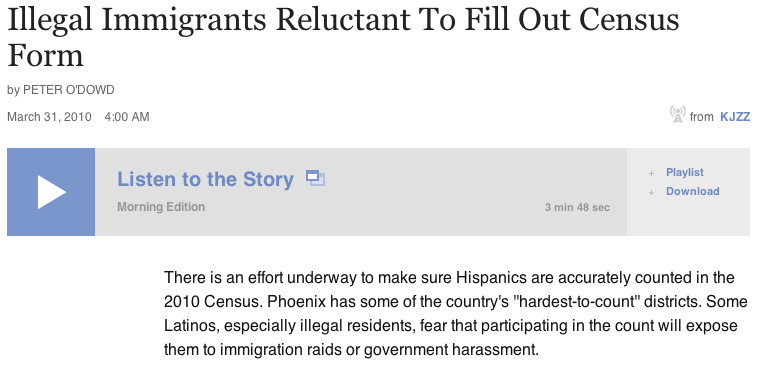
\includegraphics[width=0.90\textwidth]{../../Chp 1/1-3_sampling_principles_strategies/figures/census_illegal_immig}
\end{center}

\ct{\webURL{http://www.npr.org/templates/story/story.php?storyId=125380052}}

\end{frame}

%%%%%%%%%%%%%%%%%%%%%%%%%%%%%%%%%%%%%

\begin{frame}
\frametitle{Exploratory analysis to inference}

\begin{itemize}

\item Sampling is natural.

\pause

\item Think about sampling something you are cooking - you taste (examine) a small part of what you're cooking to get an idea about the dish as a whole.

\pause

\item When you taste a spoonful of soup and decide the spoonful you tasted isn't salty enough, that's \hl{exploratory analysis}.

\pause

\item If you generalize and conclude that your entire soup needs salt, that's an \hl{inference}.

\pause

\item For your inference to be valid, the spoonful you tasted (the sample) needs to be \hl{representative} of the entire pot (the population).

\begin{itemize}
\item If your spoonful comes only from the surface and the salt is collected at the bottom of the pot, what you tasted is probably not representative of the whole pot.
\item If you first stir the soup thoroughly before you taste, your spoonful will more likely be representative of the whole pot.
\end{itemize}

\end{itemize}

\end{frame}

%%%%%%%%%%%%%%%%%%%%%%%%%%%%%%%%%%%%

\begin{frame}
\frametitle{Sampling bias}

\begin{itemize}

\item \hl{Non-response:} If only a small fraction of the randomly sampled people choose to respond to a survey, the sample may no longer be representative of the population.

\pause

\item \hl{Voluntary response:} Occurs when the sample consists of people who volunteer to respond because they have strong opinions on the issue. Such a sample will also not be representative of the population.

\pause

\begin{center}
%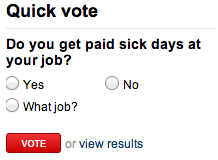
\includegraphics[width=0.25\textwidth]{../../Chp 1/1-3_sampling_principles_strategies/figures/vol_resp_bias/vol_resp_bias_q}\pause
%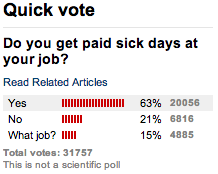
\includegraphics[width=0.25\textwidth]{../../Chp 1/1-3_sampling_principles_strategies/figures/vol_resp_bias/vol_resp_bias_res} \\
{\tiny cnn.com, Jan 14, 2012}
\end{center}

\pause

\item \hl{Convenience sample:} Individuals who are easily accessible are more likely to be included in the sample.

\end{itemize}

\end{frame}

%%%%%%%%%%%%%%%%%%%%%%%%%%%%%%%%%%%%

\begin{frame}
\frametitle{Sampling bias example: Landon vs. FDR}

A historical example of a biased sample yielding misleading results: \\

$\:$ \\

\begin{columns}[c]

\column{0.35\textwidth}

%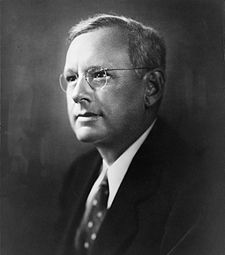
\includegraphics[width= \textwidth]{../../Chp 1/1-3_sampling_principles_strategies/figures/landon_fdr/landon}

\column{0.3\textwidth}
In 1936, Landon sought the Republican presidential nomination opposing the re-election of FDR.

\column{0.35\textwidth}

%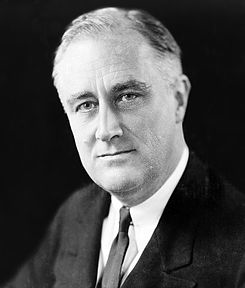
\includegraphics[width= \textwidth]{../../Chp 1/1-3_sampling_principles_strategies/figures/landon_fdr/fdr}

\end{columns}

\end{frame}

%%%%%%%%%%%%%%%%%%%%%%%%%%%%%%%%%%%%%

\begin{frame}
\frametitle{The Literary Digest Poll}

\begin{columns}

\column{0.7\textwidth}

\begin{itemize}

\item The Literary Digest polled about 10 million Americans, and got responses from about 2.4 million.

\item The poll showed that Landon would likely be the overwhelming winner and FDR would get only 43\% of the votes.

\item Election result:  FDR won, with 62\% of the votes.

\end{itemize}

\column{0.3\textwidth}

%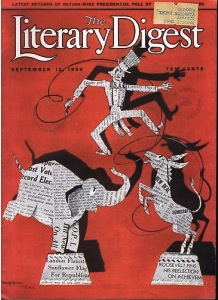
\includegraphics[width= \textwidth]{../../Chp 1/1-3_sampling_principles_strategies/figures/literaryDigest}

\end{columns}

\begin{itemize}

\item The magazine was completely discredited because of the poll, and was soon discontinued.

\end{itemize}

\end{frame}

%%%%%%%%%%%%%%%%%%%%%%%%%%%%%%%%%%%%%

\begin{frame}
\frametitle{The Literary Digest Poll -- what went wrong?}

\begin{itemize}

\item The magazine had surveyed

\begin{itemize}

\item its own readers,

\item registered automobile owners, and

\item registered telephone users.

\end{itemize}

\item These groups had incomes well above the national average of the day (remember, this is Great Depression era) which resulted in lists of voters far more likely to support Republicans than a truly \hl{typical} voter of the time, i.e. the sample was not representative of the American population at the time.

\end{itemize}

\end{frame}

%%%%%%%%%%%%%%%%%%%%%%%%%%%%%%%%%%%%%

\begin{frame}
\frametitle{Large samples are preferable, but...}

\begin{itemize}

\item The Literary Digest election poll was based on a sample size of 2.4 million, which is huge, but since the sample was \hl{biased}, the sample did not yield an accurate prediction.

\item Back to the soup analogy: If the soup is not well stirred, it doesn't matter how large a spoon you have, it will still not taste right. If the soup is well stirred, a small spoon will suffice to test the soup.

\end{itemize}

\end{frame}

%%%%%%%%%%%%%%%%%%%%%%%%%%%%%%%%%%%%%

\begin{frame}[shrink]
\frametitle{Practice}

{\small
\pq{A school district is considering whether it will no longer allow high school students to park at school after two recent accidents where students were severely injured. As a first step, they survey parents by mail, asking them whether or not the parents would object to this policy change. Of 6,000 surveys that go out, 1,200 are returned. Of these 1,200 surveys that were completed, 960 agreed with the policy change and 240 disagreed. Which of the following statements are true?}

\begin{enumerate}[I.]
\item Some of the mailings may have never reached the parents.
\item The school district has strong support from parents to move forward with the policy approval.
\item It is possible that majority of the parents of high school students disagree with the policy change.
\item The survey results are unlikely to be biased because all parents were mailed a survey. 
\end{enumerate}

\begin{multicols}{5}
\begin{enumerate}[(a)]
\item Only I
\item I and II
\solnMult{I and III}
\item III and IV
\item Only IV
\end{enumerate}
\end{multicols}
}

\end{frame}

%%%%%%%%%%%%%%%%%%%%%%%%%%%%%%%%%%%%%

\subsection{Observational studies}

%%%%%%%%%%%%%%%%%%%%%%%%%%%%%%%%%%%%%

\begin{frame}
\frametitle{Observational studies}

\begin{itemize}

\item Researchers collect data in a way that does not directly interfere with how the data arise.

\item Results of an observational study can generally be used to establish an association between the explanatory and response variables.

\end{itemize}

\end{frame}

%%%%%%%%%%%%%%%%%%%%%%%%%%%%%%%%%%%%%

\subsection{Four sampling methods}

%%%%%%%%%%%%%%%%%%%%%%%%%%%%%%%%%%%%%

\begin{frame}
\frametitle{Obtaining good samples}

\begin{itemize}

\item Almost all statistical methods are based on the notion of implied randomness. 

\item If observational data are not collected in a random framework from a population, these statistical methods -- the estimates and errors associated with the estimates -- are not reliable.

\item Most commonly used random sampling techniques are \hl{simple}, \hl{stratified}, and \hl{cluster} sampling.

\end{itemize}

\end{frame}

%%%%%%%%%%%%%%%%%%%%%%%%%%%%%%%%%%%%

\begin{frame}
\frametitle{Simple random sample}

Randomly select cases from the population, where there is no implied connection between the points that are selected.

\begin{center}
%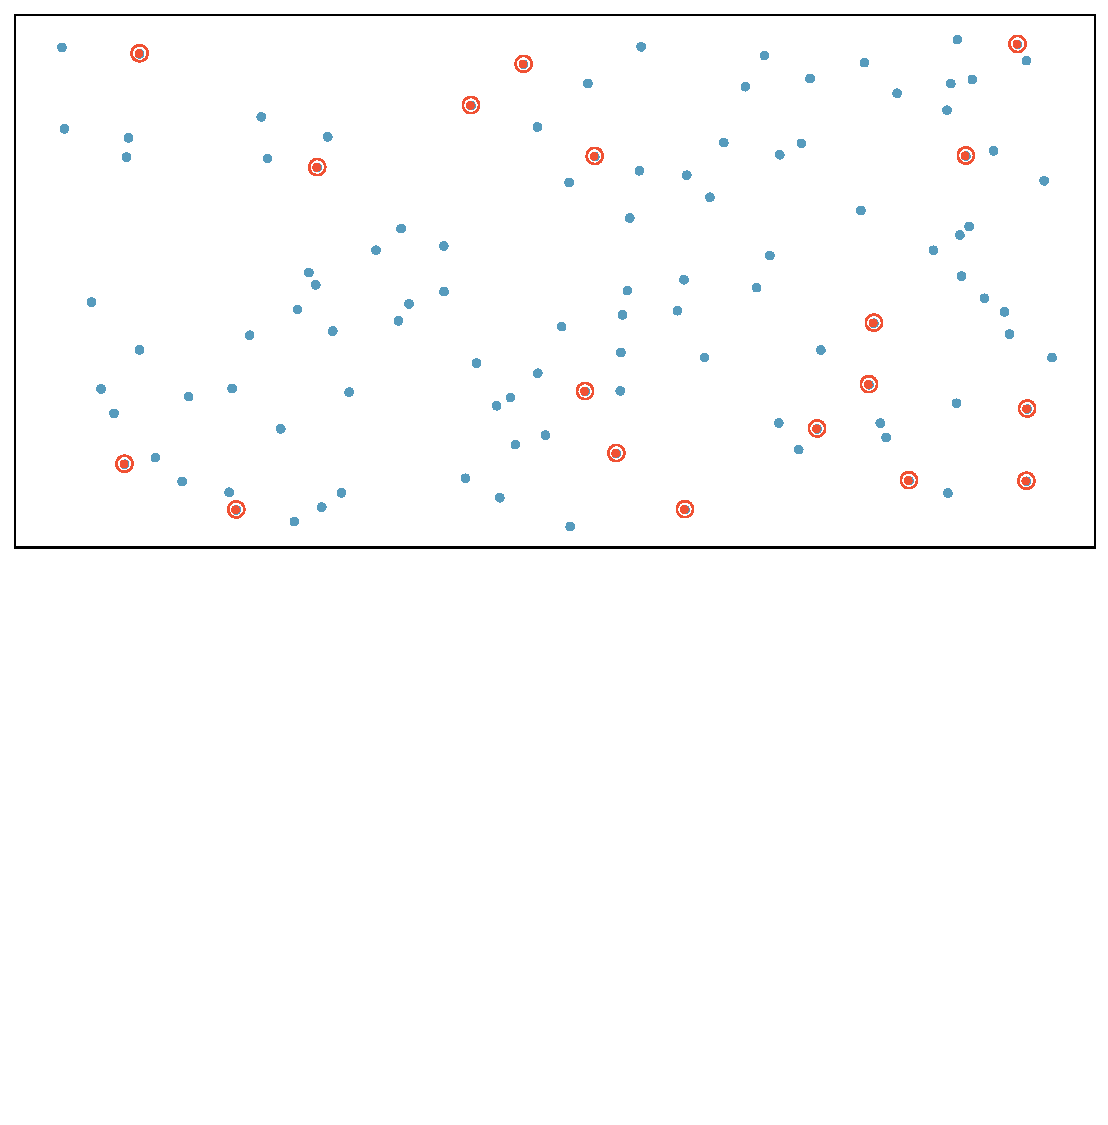
\includegraphics[width=0.9\textwidth]{../../Chp 1/1-3_sampling_principles_strategies/figures/sampling_methods/simple}
\end{center}

\end{frame}

%%%%%%%%%%%%%%%%%%%%%%%%%%%%%%%%%%%%

\begin{frame}
\frametitle{Stratified sample}

\hl{Strata} are made up of similar observations. We take a simple random sample from \underline{each} stratum.

\begin{center}
%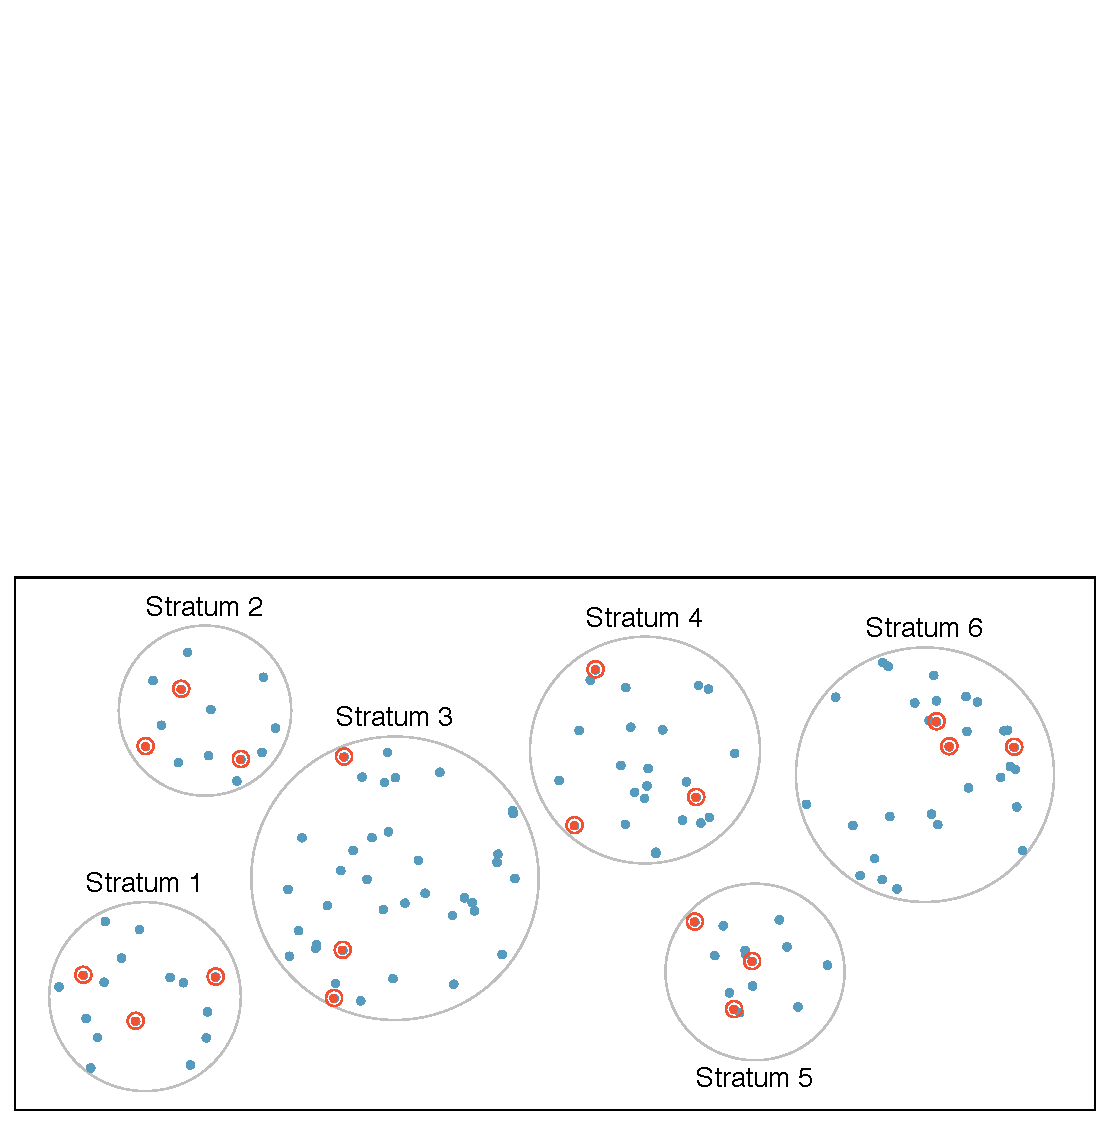
\includegraphics[width=0.9\textwidth]{../../Chp 1/1-3_sampling_principles_strategies/figures/sampling_methods/stratified}
\end{center}

\end{frame}

%%%%%%%%%%%%%%%%%%%%%%%%%%%%%%%%%%%%

\begin{frame}
\frametitle{Cluster sample}

\hl{Clusters} are usually not made up of homogeneous observations. We take a simple random sample of clusters, and then sample \underline{all} observations in that cluster. Usually preferred for economical reasons.

\begin{center}
%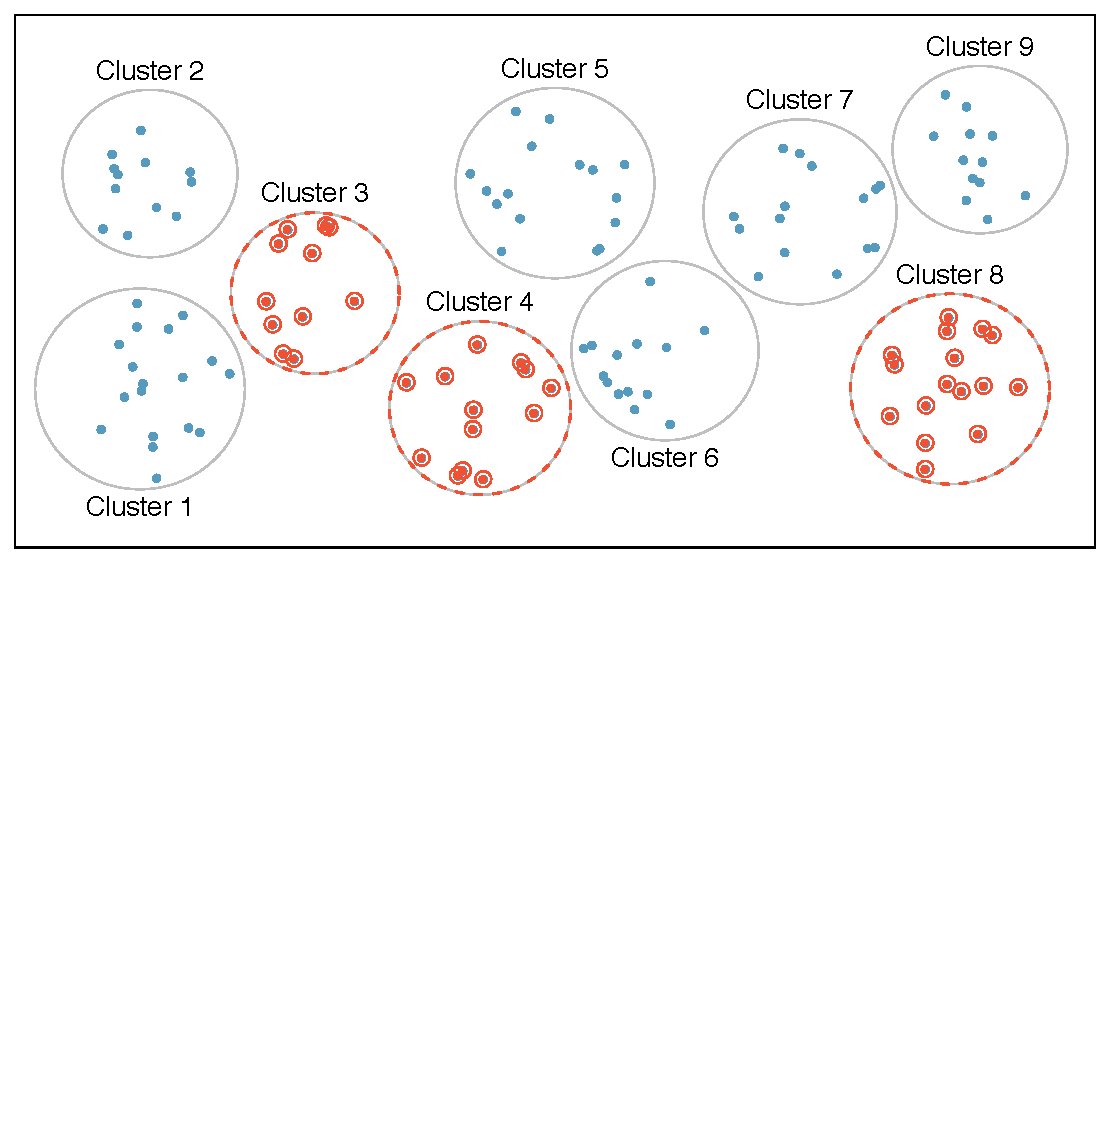
\includegraphics[width=0.9\textwidth]{../../Chp 1/1-3_sampling_principles_strategies/figures/sampling_methods/cluster}
\end{center}

\end{frame}

%%%%%%%%%%%%%%%%%%%%%%%%%%%%%%%%%%%%

\begin{frame}
\frametitle{Multistage sample}

\hl{Clusters} are usually not made up of homogeneous observations.  We take a simple random sample of clusters, and then take a simple random sample of observations from the sampled clusters.

\begin{center}
%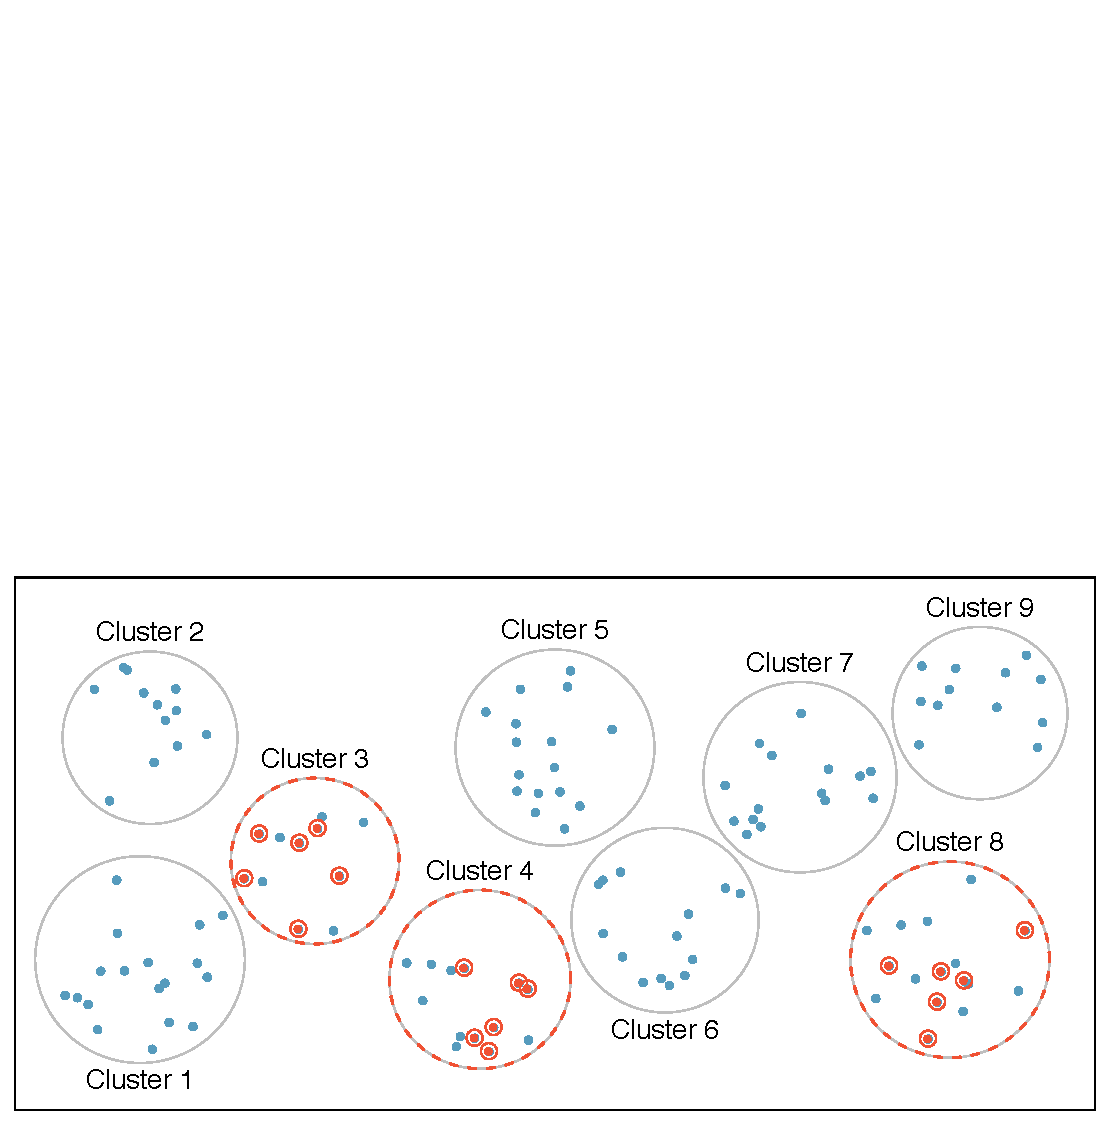
\includegraphics[width=0.9\textwidth]{../../Chp 1/1-3_sampling_principles_strategies/figures/sampling_methods/multistage}
\end{center}

\end{frame}

%%%%%%%%%%%%%%%%%%%%%%%%%%%%%%%%%%%%

\begin{frame}
\frametitle{Practice}

\pq{A city council has requested a household survey be conducted in a suburban area of their city. The area is broken into many distinct and unique neighborhoods, some including large homes, some with only apartments. Which approach would likely be the \emph{least} effective?}

\begin{enumerate}[(a)]
\item Simple random sampling
\solnMult{Cluster sampling}
\item Stratified sampling
\item Blocked sampling
\end{enumerate}

\end{frame}

%%%%%%%%%%%%%%%%%%%%%%%%%%%%%%%%%%%%

%%%%%%%%%%%%%%%%%%%%%%%%%%%%%%%%%%%%

\section{Experiments}

%%%%%%%%%%%%%%%%%%%%%%%%%%%%%%%%%%%%

\begin{frame}
\frametitle{Principles of experimental design}

\begin{enumerate}

\item \hl{Control:} Control for the (potential) effect of variables other than the ones directly being studied.

\item \hl{Randomize:} Randomly assign subjects to treatments, and randomly sample from the population whenever possible.

\item \hl{Replicate:} Within a study, replicate by collecting a sufficiently large sample. Or replicate the entire study.

\item \hl{Block:} If there are variables that are known or suspected to affect the response variable, first group subjects into \hl{blocks} based on these variables, and then randomize cases within each block to treatment groups.

\end{enumerate}

\end{frame}

%%%%%%%%%%%%%%%%%%%%%%%%%%%%%%%%%%%%

\begin{frame}
\frametitle{More on blocking}


\twocol{0.25}{0.75}
{
\begin{center}
%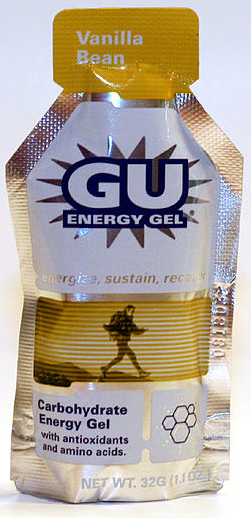
\includegraphics[width=\textwidth]{../../Chp 1/1-4_experiments/figures/gu}
\end{center}
}
{
\begin{itemize}
\item We would like to design an experiment to investigate if energy gels makes you run faster:

\pause

\begin{itemize}
\item Treatment: energy gel
\item Control: no energy gel
\end{itemize}

\pause

\item It is suspected that energy gels might affect pro and amateur athletes differently, therefore we block for pro status:

\pause

\begin{itemize}
\item Divide the sample to pro and amateur
\item Randomly assign pro athletes to treatment and control groups
\item Randomly assign amateur athletes to treatment and control groups
\item Pro/amateur status is equally represented in the resulting treatment and control groups
\end{itemize}
\end{itemize}
}

\pause

\dq{Why is this important? Can you think of other variables to block for?}

\end{frame}

%%%%%%%%%%%%%%%%%%%%%%%%%%%%%%%%%%%%

\begin{frame}
\frametitle{Practice}

\pq{A study is designed to test the effect of light level and noise level on exam performance of students. The researcher also believes that light and noise levels might have different effects on males and females, so wants to make sure both genders are equally represented in each group. Which of the below is correct?}

\begin{enumerate}[(a)]
\item There are 3 explanatory variables (light, noise, gender) and 1 response variable (exam performance)
\solnMult{There are 2 explanatory variables (light and noise), 1 blocking variable (gender), and 1 response variable (exam performance)}
\item There is 1 explanatory variable (gender) and 3 response variables (light, noise, exam performance)
\item There are 2 blocking variables (light and noise), 1 explanatory variable (gender), and 1 response variable (exam performance)
\end{enumerate}

\end{frame}

%%%%%%%%%%%%%%%%%%%%%%%%%%%%%%%%%%%%

\begin{frame}
\frametitle{Difference between blocking and explanatory variables}

\begin{itemize}

\item Factors are conditions we can impose on the experimental units.

\item Blocking variables are characteristics that the experimental units come with, that we would like to control for.

\item Blocking is like stratifying, except used in experimental settings when randomly assigning, as opposed to when sampling.

\end{itemize}

\end{frame}

%%%%%%%%%%%%%%%%%%%%%%%%%%%%%%%%%%%%

\begin{frame}
\frametitle{More experimental design terminology...}

\begin{itemize}

\item \hl{Placebo:} fake treatment, often used as the control group for medical studies

\item \hl{Placebo effect:} experimental units showing improvement simply because they believe they are receiving a special treatment

\item \hl{Blinding:} when experimental units do not know whether they are in the control or treatment group

\item \hl{Double-blind:} when both the experimental units and the researchers who interact with the patients do not know who is in the control and who is in the treatment group

\end{itemize}

\end{frame}

%%%%%%%%%%%%%%%%%%%%%%%%%%%%%%%%%%%%

\begin{frame}
\frametitle{Practice}

\pq{What is the main difference between observational studies and experiments?}

\begin{enumerate}[(a)]
\item Experiments take place in a lab while observational studies do not need to.
\item In an observational study we only look at what happened in the past.
\solnMult{Most experiments use random assignment while observational studies do not.}
\item Observational studies are completely useless since no causal inference can be made based on their findings.
\end{enumerate}

\end{frame}

%%%%%%%%%%%%%%%%%%%%%%%%%%%%%%%%%%%%

\begin{frame}
\frametitle{Random assignment vs. random sampling}

\begin{center}
%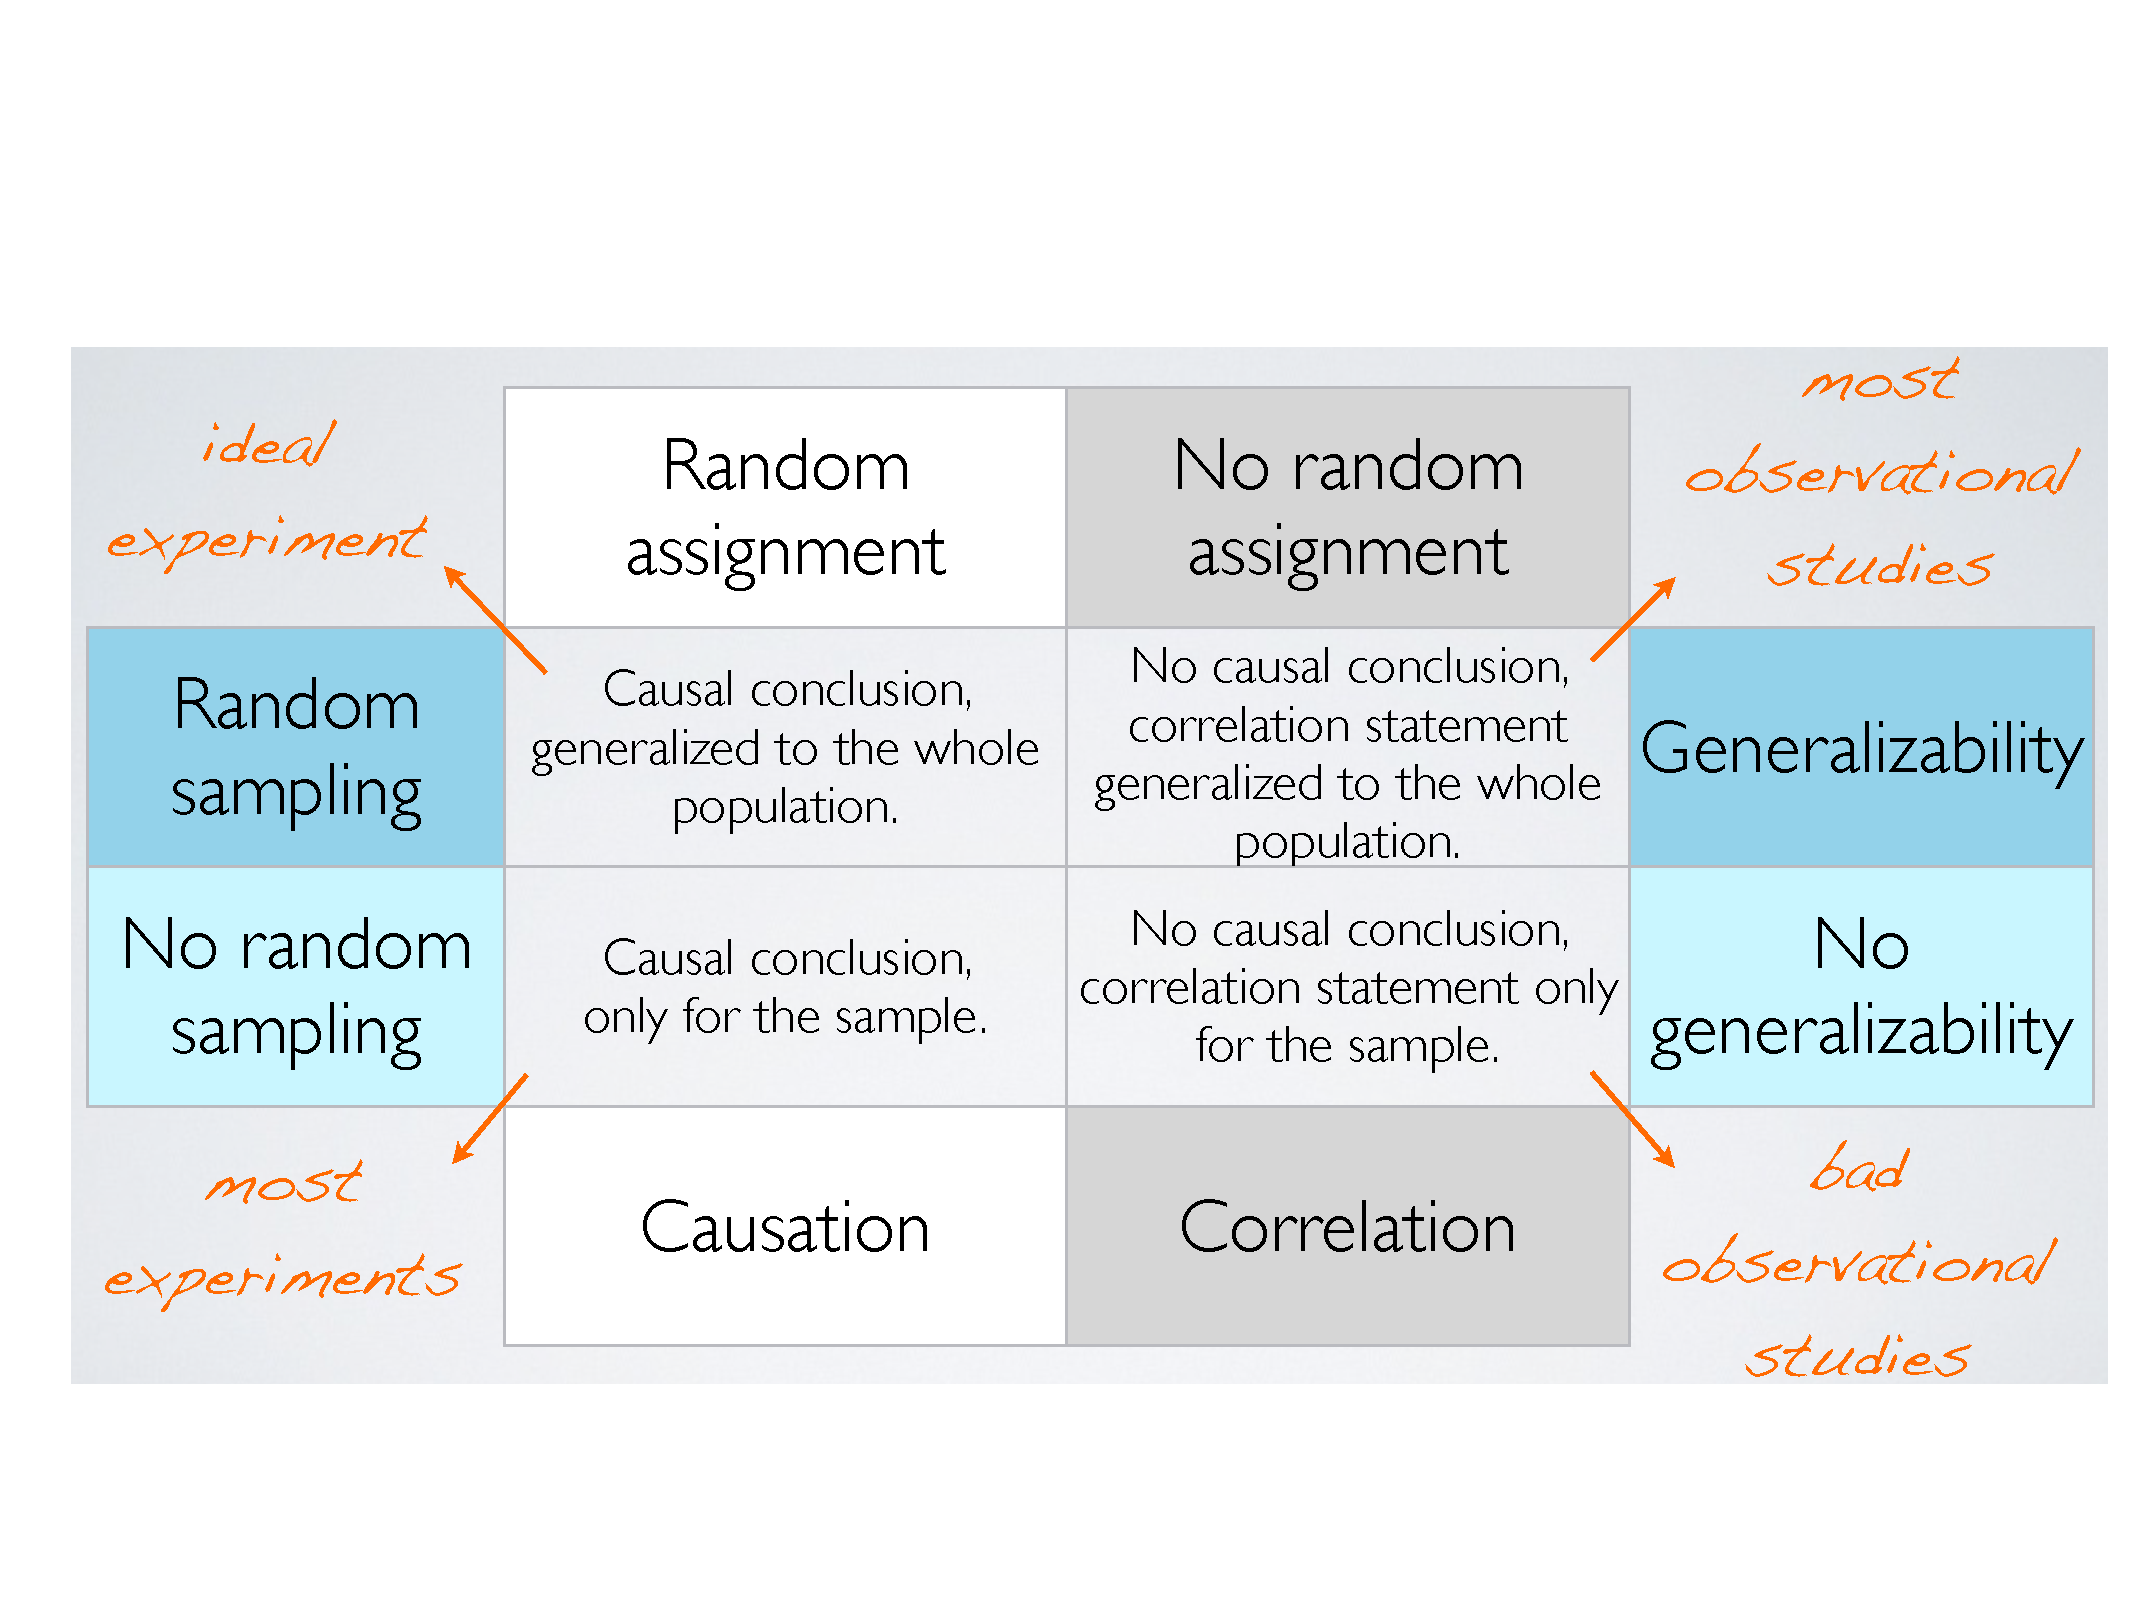
\includegraphics[width=\textwidth]{../../Chp 1/1-4_experiments/figures/random_sample_assignment}
\end{center}

\end{frame}

%%%%%%%%%%%%%%%%%%%%%%%%%%%%%%%%%%%%


%%%%%%%%%%%%%%%%%%%%%%%%%%%%%%%%%%%%
% End document
%%%%%%%%%%%%%%%%%%%%%%%%%%%%%%%%%%%%

\end{document}